\documentclass[12pt,a4paper]{article}

\usepackage[lmargin=2cm, rmargin=2cm, tmargin=2cm, bmargin=2cm]{geometry}

%\usepackage[polish]{babel}
\usepackage[latin2]{inputenc}
\usepackage[OT4]{fontenc}

\usepackage{sectsty}
\usepackage[usenames]{color}

\usepackage{listings} % http://www.pvv.ntnu.no/~berland/latex/docs/listings.pdf
\usepackage{fancyvrb}

\usepackage{graphicx} % \includegraphics[scale=0.5]{img/temperature.png}

\usepackage[pdftex,colorlinks=true,urlcolor=blue,pdfusetitle=true]{hyperref} 

\newcommand{\HRule}{\rule{\linewidth}{0.5mm}}

\hypersetup{
pdfkeywords={tutorial, python, django}
}

% \tiny
% \scriptsize
% \footnotesize
% 
% \small
% \Large
% \LARGE
% \large
% \huge
% \Huge

\renewcommand\familydefault{\sfdefault}

\sectionfont{\normalsize} 
\subsectionfont{\normalsize}
\definecolor{gray}{gray}{0.4}

\lstdefinelanguage{sdgen}{
        morekeywords = {children, type, value, view, name},
        keywordstyle=\color{blue}\bfseries,
        basicstyle=\scriptsize\ttfamily,
        frame = lines
}
\lstset{language=sdgen}

\newcommand{\chapter}[1]{\section*{\Large#1}\setcounter{section}{0}}

%%%%%%%%%%%%%%%%%%%%%%%%%%%%%%%%%%%%%%%%%
% >>>>>>>>>>>>>>>>>>>>>>>>>
\begin{document}
% >>>>>>>>>>>>>>>>>>>>>>>>>

\begin{titlepage}
\vspace*{\fill}
\begin{center}

%\textsc{\Large Python project for Technologies of Software Development}\\[0.5cm]


% Title
\HRule \\[0.4cm]
{ \huge \bfseries Syntax Diagram Generator}\\[0.4cm]

\HRule \\[1.5cm]

% Author and supervisor
%\emph{Supervisor:} 
%\begin{itemize}
%\item Bartosz \textsc{Alchimowicz}, M.Sc.
%\end{itemize}

%\emph{Authors:}
%\begin{itemize}
%\item Mariano \textsc{Calderon Arenas} 
%\item Pawel \textsc{Radzikowski} 
%\item Jakub \textsc{Rojek} 
%\end{itemize}
%\vfill

% Bottom of the page
{\large \today}
\end{center}
\vspace*{\fill}

\end{titlepage}



%%%%%%%%%%%%%%%%%%
\chapter{Short description}
%%%%%%%%%%%%%%%%%%

Syntax Diagram Generator is an application written in Python which convert definition of diagram (in structured form) to SVG image(s). 

%%%%%%%%%%%%%%%%%%
\chapter{Getting started}
%%%%%%%%%%%%%%%%%%

\section{Installation}

Before start using Syntax Diagram Generator, user should assure that specific libraries and packages have been installed in a operation system:

\begin{itemize}
\item setuptools (\url{http://pypi.python.org/pypi/setuptools})
\item pysvg (\url{http://pypi.python.org/pypi/pysvg/0.2.1})
\item CairoSVG (\url{http://cairosvg.org/})
\item python-tk (\url{http://wiki.python.org/moin/TkInter})
\end{itemize} 

\noindent
After satisfy these assumptions, installation of Syntax Diagram Generator is executing the command:
\newline
\newline
\texttt{python setup.py install}
\section{Running an application}

To get a SVG diagram, a appriopriate Python file should be prepared:

\begin{lstlisting}[caption={Example of input Python file}]
# -*- coding: utf-8 -*-
import sys
sys.path.append('.')
from sdgen.svg import *

#definition of diagram
#examples will appear in the next chapter
data = {
	...
}

#a second parameter tells about directory
#to write all diagrams
result = as_svg(data, 'directory')
#printing resulting main image
#first index - number of image
#second index - 0 for name, 1 for data
print result[0][1].encode('utf-8')
\end{lstlisting}

\noindent
Then generating a image (or images) is executing a command:
\newline
\newline
\texttt{python examples/inputfile.py directory $>$ outputimage.svg}
\newline
\newline
All images will be deployed into the specified directory and the main image into \texttt{outputimage.svg} file.

%%%%%%%%%%%%%%%%%%
\chapter{Examples}
%%%%%%%%%%%%%%%%%%
\section{Terminal example}
%%%%%%%%%%%%%%%%%%

\lstinputlisting[caption={Terminal example}]{examples/onlyinputs/ex01.py}

\begin{figure}[h!]
\caption{Output for listing 2}
\centering
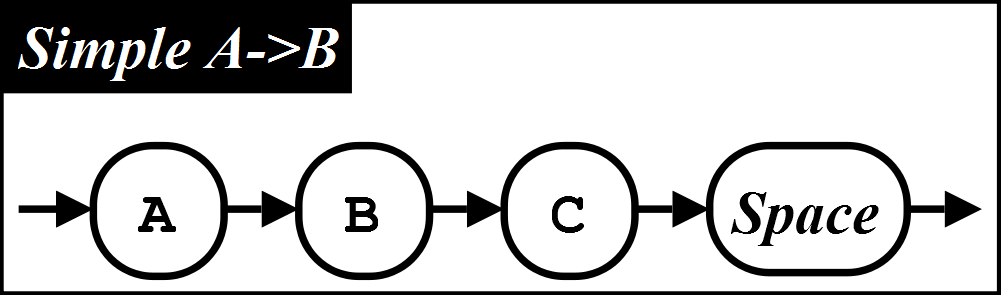
\includegraphics[width=0.3\textwidth]{results/ex01.png}
\end{figure}

%%%%%%%%%%%%%%%%%%
\section{Sequence example}
%%%%%%%%%%%%%%%%%%

\lstinputlisting[caption={Sequence example}]{examples/onlyinputs/ex05.py}

\begin{figure}[h!]
\caption{Output for listing 3}
\centering
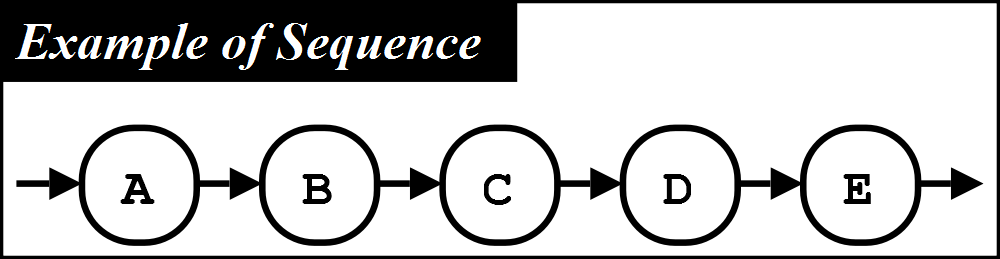
\includegraphics[width=0.5\textwidth]{results/ex05.png}
\end{figure}

\pagebreak

%%%%%%%%%%%%%%%%%%
\section{Return example}
%%%%%%%%%%%%%%%%%%

\lstinputlisting[caption={Return example}]{examples/onlyinputs/ex07.py}

\begin{figure}[h!]
\caption{Output for listing 4}
\centering
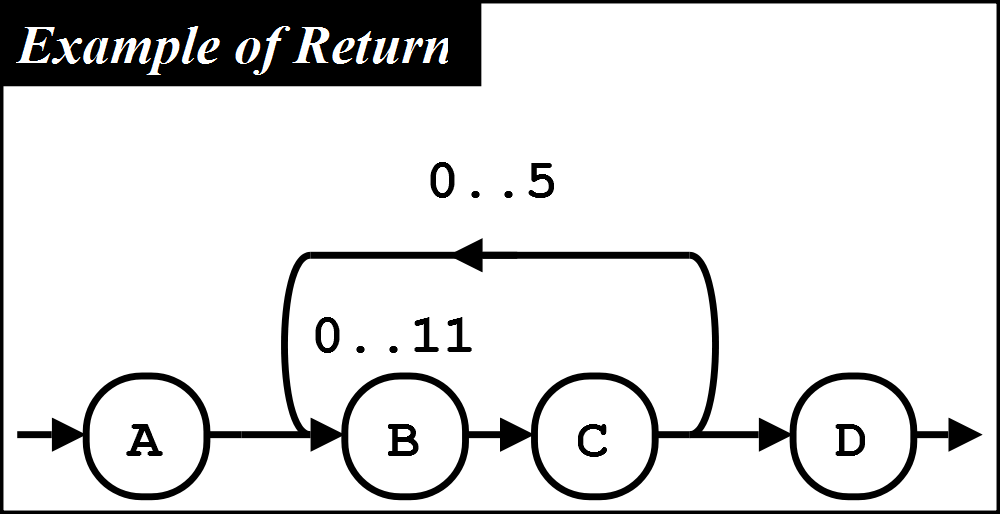
\includegraphics[width=0.5\textwidth]{results/ex07.png}
\end{figure}

%%%%%%%%%%%%%%%%%%
\section{Alternation example}
%%%%%%%%%%%%%%%%%%

\lstinputlisting[caption={Alternation example}]{examples/onlyinputs/ex06.py}

\begin{figure}[h!]
\caption{Output for listing 5}
\centering
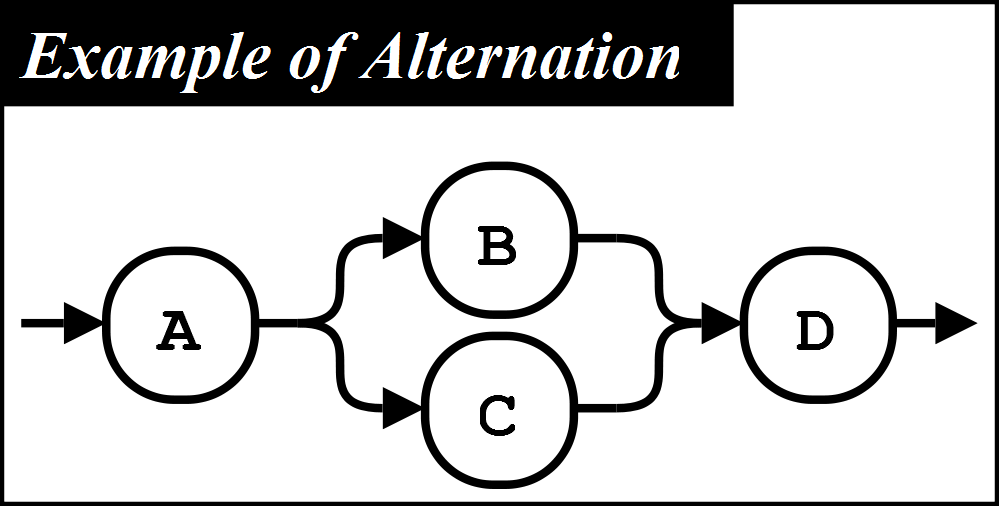
\includegraphics[width=0.5\textwidth]{results/ex06.png}
\end{figure}

%%%%%%%%%%%%%%%%%%
\section{Detour example}
%%%%%%%%%%%%%%%%%%

\lstinputlisting[caption={Detour example}]{examples/onlyinputs/ex02b.py}

\begin{figure}[h!]
\caption{Output for listing 6}
\centering
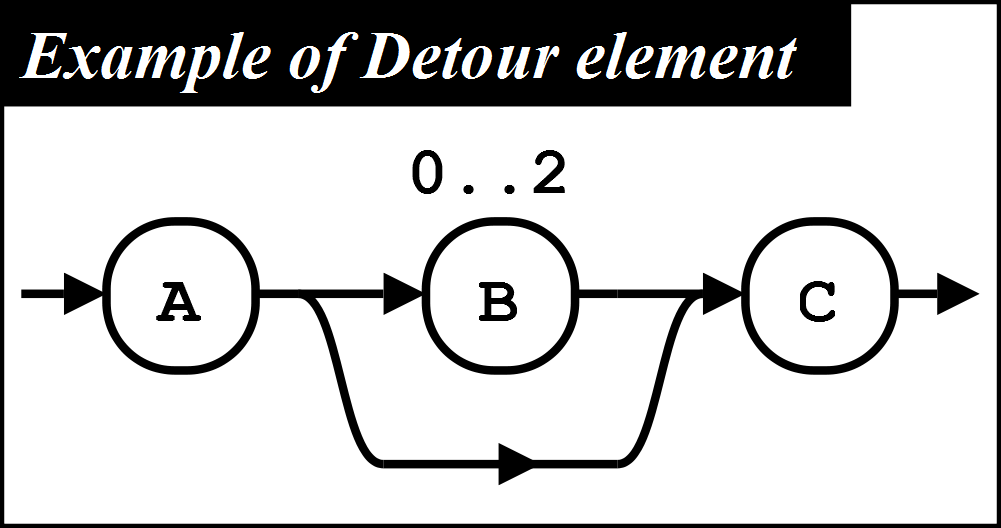
\includegraphics[width=0.5\textwidth]{results/ex02.png}
\end{figure}

%%%%%%%%%%%%%%%%%%
\section{Inverse terminal example}
%%%%%%%%%%%%%%%%%%

\lstinputlisting[caption={Inverse terminal example}]{examples/onlyinputs/ex04.py}

\begin{figure}[h!]
\caption{Output for listing 7}
\centering
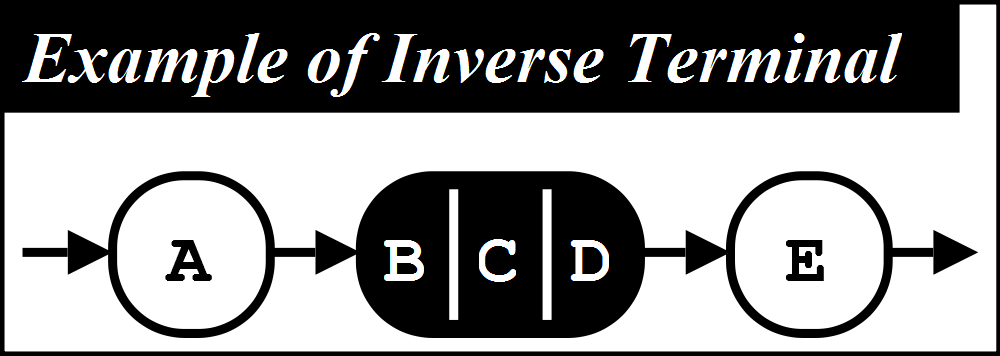
\includegraphics[width=0.5\textwidth]{results/ex04.png}
\end{figure}

%%%%%%%%%%%%%%%%%%
\section{Nonterminal example}
%%%%%%%%%%%%%%%%%%

\lstinputlisting[caption={Nonterminal example}]{examples/onlyinputs/ex03.py}

\begin{figure}[h!]
\caption{Output for listing 8}
\centering
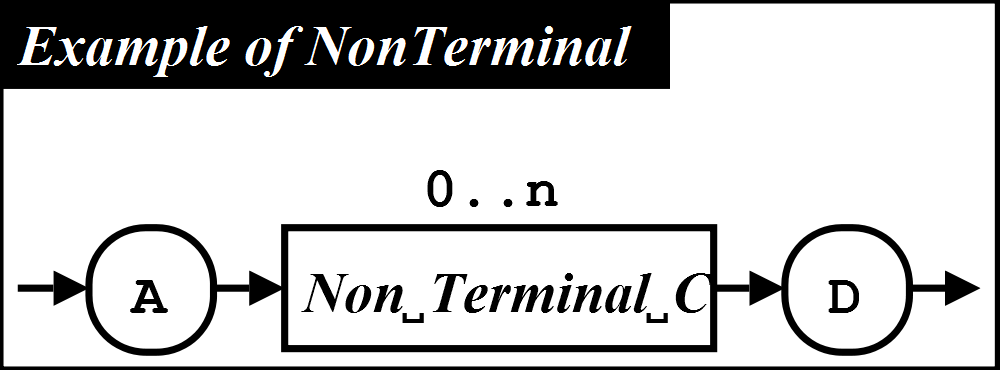
\includegraphics[width=0.5\textwidth]{results/ex03a.png}
\end{figure}

\begin{figure}[h!]
\caption{Output for listing 8 (internal subimage)}
\centering
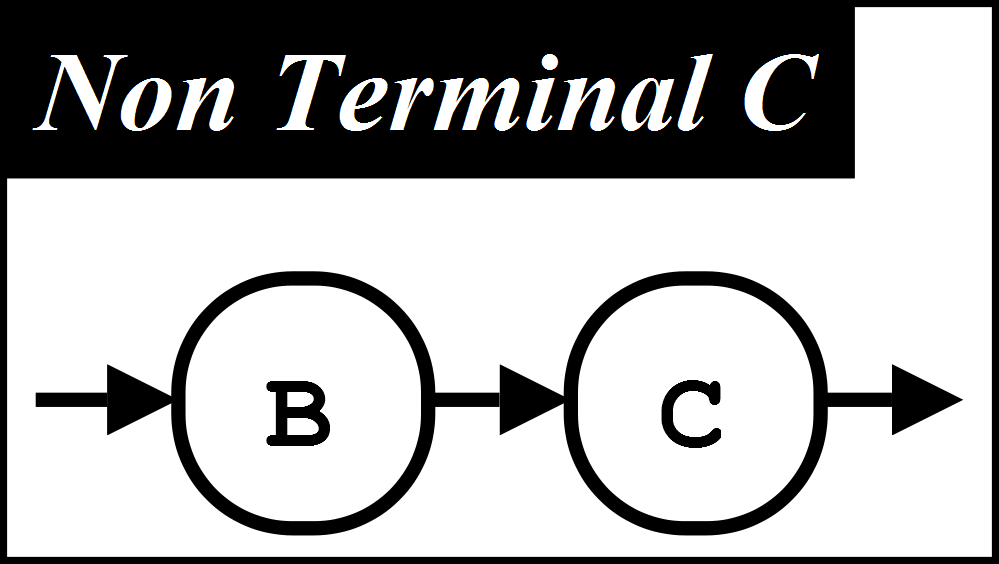
\includegraphics[width=0.3\textwidth]{results/ex03b.png}
\end{figure}

%%%%%%%%%%%%%%%%%%
\section{Nested groups example}
%%%%%%%%%%%%%%%%%%

\lstinputlisting[caption={Nested groups example}]{examples/onlyinputs/ex09.py}

\begin{figure}[h!]
\caption{Output for listing 9}
\centering
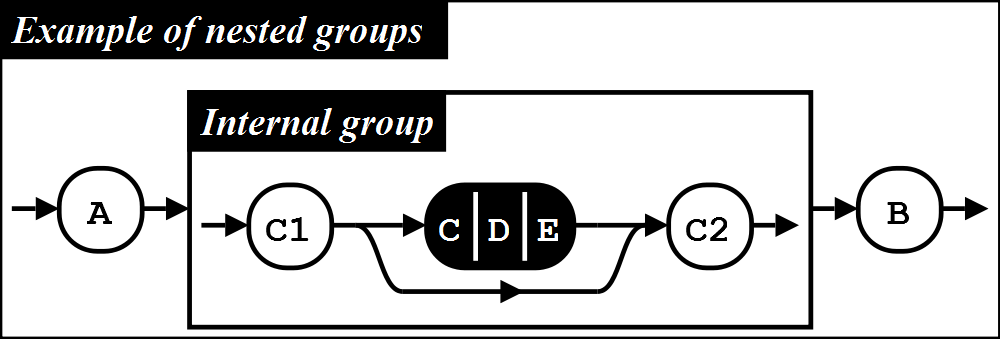
\includegraphics[width=0.8\textwidth]{results/ex09.png}
\end{figure}

% <<<<<<<<<<<<<<<<<<<<<<<<<
\end{document}
% <<<<<<<<<<<<<<<<<<<<<<<<<

